\chapter{Satellite Modeling}

\section{Reference Frames}

\nomenclature[A]{\textbf{ECI}}{Earth Centered Inertial Frame}
\nomenclature[A]{\textbf{ECEF}}{Earth Centered Earth Fixed Frame}
\nomenclature[A]{\textbf{SBRF}}{Satellite Body Reference Frame}

Using different reference frame for different calculations can simplify equations. Values in one reference frame can be converted into the other by using the proper transformations.
Inertial frames of reference are frames where Newton's 3 laws of dynamics apply.
The most used reference frames for Earth-orbiting satellites are Earth Centered Inertial Frame (ECI), Earth Centered Earth Fixed Frame (ECEF), Orbit Frame, Satellite Body Reference Frame (SBRF)  \cite{ref1} \cite{ref2}. Figure \ref{fig:frames} provides a visualization of the frames.

\begin{figure}[h!]
	\centering 
	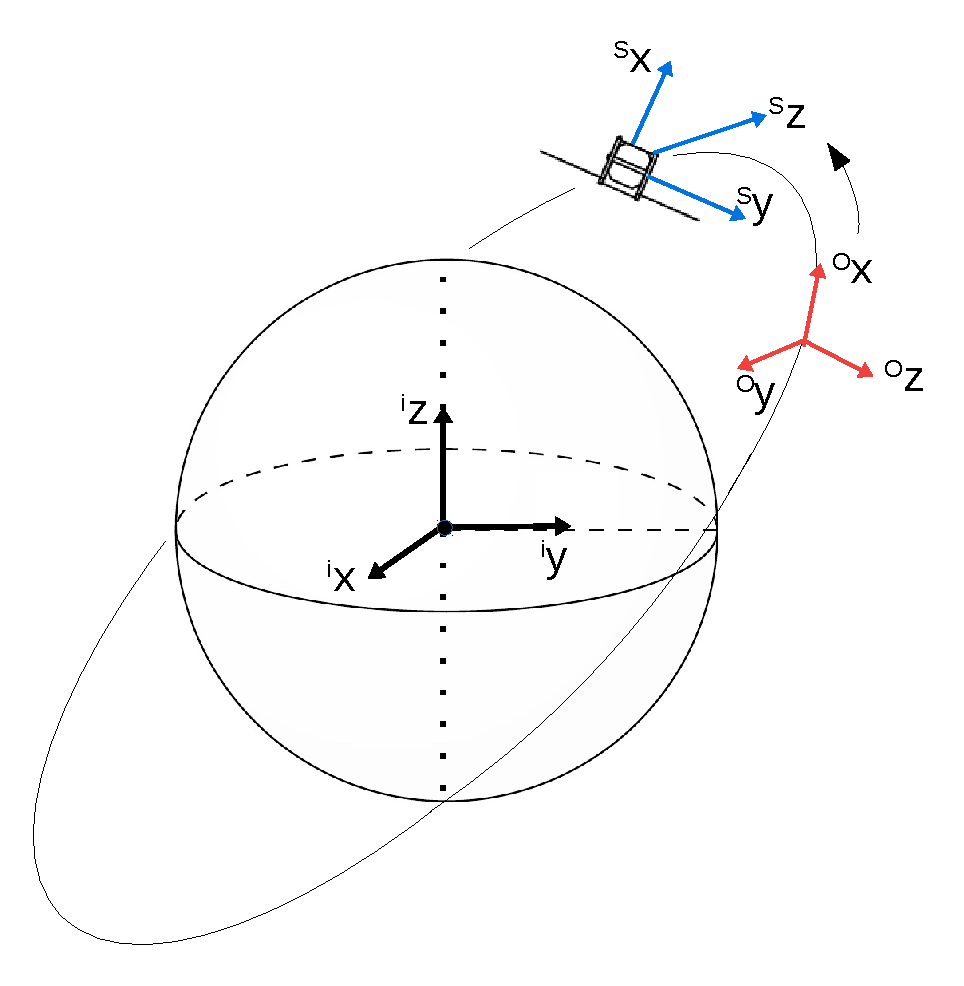
\includegraphics[width=140mm]{figures/frame.pdf}	
	\caption{Reference frame axes. Superscripts: i - ECI, o - Orbital, s - Satellite Body Frame \cite{our_report}.}
	\label{fig:frames}
\end{figure}

\subsubsection{Earth Centered Inertial Frame (ECI)}
Earth is rotating and is orbiting the Sun, it accelerates in the direction of the Sun's center of mass, the Sun is orbiting the center of the Milky Way, etc. Thus there is no frame fixed to Earth's center that is an inertial frame \textit{per definitionem}. But in the case of earth orbiting satellites, there exists a coordinate system attached to Earth's center that out of practical considerations can be treated as one, the Earth Centered Inertial Frame (ECI).
As the name suggests, the origin of the coordinate system is the center of earth. Inertial means that the frame doesn't rotate, the direction of stars remain the same. 
ECI is a cartesian coordinate system. Its $^iz$ vector points in the direction of the northern axis of rotation, while the $^ix$ axis towards the vernal equinox. The $^iy$ axis completes the triad of the right-handed Cartesian coordinate system.


\nomenclature[T]{\textbf{Vernal Equinox}}{The vernal equinox is the vector pointing towards the Sun's center during the equinox (20th of March in 2018). The $x$ vector also keeps its direction relative to the stars.}


\subsubsection{Earth Centered Earth Fixed Frame (ECEF)}

ECEF, similarly to ECI is centered at the Earth's origin. Its $z$ vector points towards the north parallel to the rotational axis. Its $x$ axis points at $0\deg$ latitude and $0\deg$ longitude on the Earth's surface, thus following Earth's rotation. This makes ECEF non-inertial. $y$ axis completes the right-handed triad.

\subsubsection{Orbital Frame}

The Orbital Frame is centered at the center of mass of the satellite. The $^oz$ axis points towards the center of Earth, $^ox$ points in the direction of the satellite's velocity, while $^oy$ is the normal vector for the orbital plane. The 3 axes make up an orthogonal triad.

\nomenclature[T]{\textbf{Nadir}}{The axis pointing towards Earth's center of mass}

\subsubsection{Satellite Body Reference Frame (SBRF)}

Body-fixed frames are attached to the satellite's body, but the orientation of the frame in relation to the body is arbitrary. Due to practical considerations the axes of the SBRF are chosen to line up with the principal axes of inertia of the body.
